\begin{frame}
\frametitle{Visualising differences}
Neuroimagers like their blobs and summary tables.

How do we best understand whole-brain multivariate differences?

Here's my attempt.....
\end{frame}


\begin{frame}
\frametitle{Exaggerated male brain}
\begin{center}
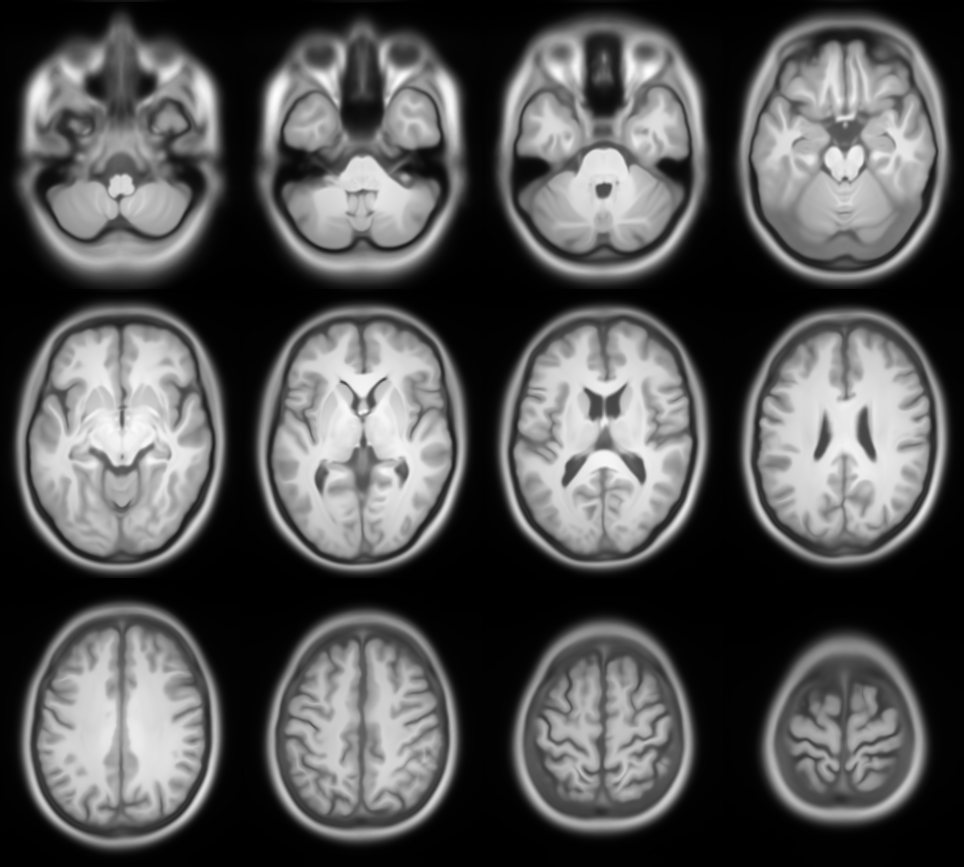
\includegraphics[width=.7\textwidth]{hyper_male}
\end{center}
\end{frame}



\begin{frame}
\frametitle{Average brain}
\begin{center}
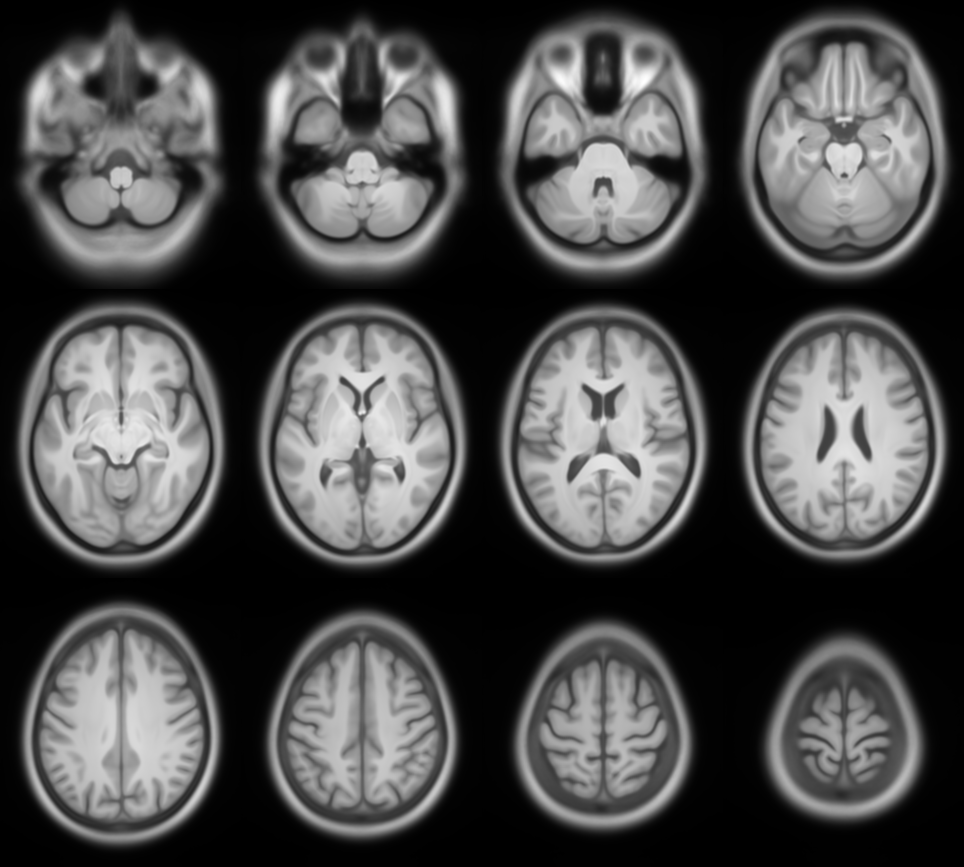
\includegraphics[width=.7\textwidth]{avgT1}
\end{center}
\end{frame}



\begin{frame}
\frametitle{Exaggerated female brain}
\begin{center}
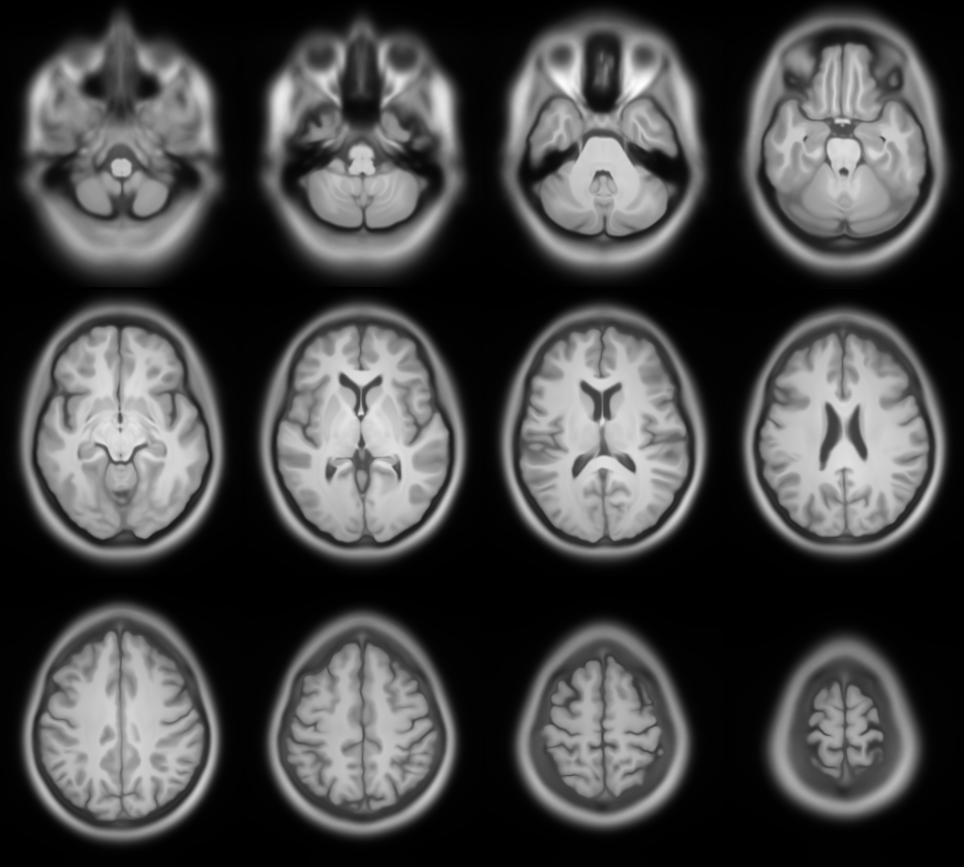
\includegraphics[width=.7\textwidth]{hyper_female}
\end{center}
\end{frame}

